\section*{Part 3}
The Figure \ref{fig:avg_em} shows the relationship of temperature with two the key properties of magnetization and energy for different sizes of square lattices.
The left columns shows the average absolute magnetization vs. temperature for each lattices size, the following observation can be made in regards to magnetization:
\begin{itemize}
	\item All three lattice size show an identical pattern, where at low temperature $T < 1$, we have high and stable magnetization (all spins point in the same direction). This is followed by a decreasing trend when increasing the temperature.
	\item The most dramatic drop in magnetization can be observed in the critical region between $2.0$ and $2.5$ for all lattice sizes. This is also where the critical temperature at $T_c = 2.27$ is located. Furthermore we can observe a steeper drop for larger lattice sizes.
	\item For temperature higher than $2.5$ the magnetization continues to decrease, but does not reach zero.
\end{itemize}
If we shift our attention to the right column, there we can make the following observations about the average energy vs. temperature plots:
\begin{itemize}
	\item For $T < 1$ all systems remain constant at minimum energy.
	\item When increasing the energy $T > 1.5$, the spins start to break the alignment with its neighbors, caused by the atoms gaining kinetic energy as temperature increases and overcoming the exchange coupling $J$.
	\item For higher temperature the system then gradually approaches to maximum disorder.
\end{itemize}
The data clearly shows a phase transition in the system around the critical temperature, which demonstrate classical behaviour of a 2D Ising model, which transitions from low temperature ordered state to a high temperature disordered state.
\begin{figure}[t]
	\centering
	\begin{subfigure}{0.5\textwidth}
		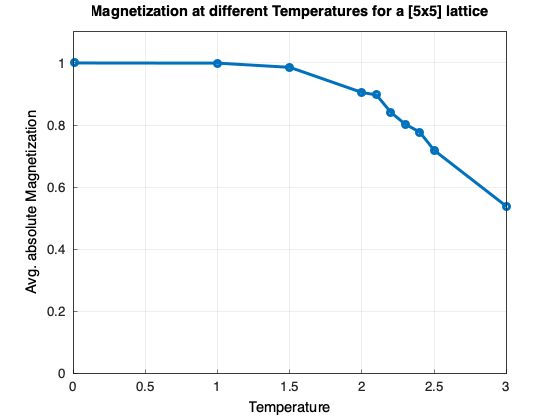
\includegraphics[width=\textwidth]{./img/avg_mag_5.png}
		\caption{$L=[5\times5]$}
		\label{sfig:sublabel1}
	\end{subfigure}%
	~
	\begin{subfigure}{0.5\textwidth}
		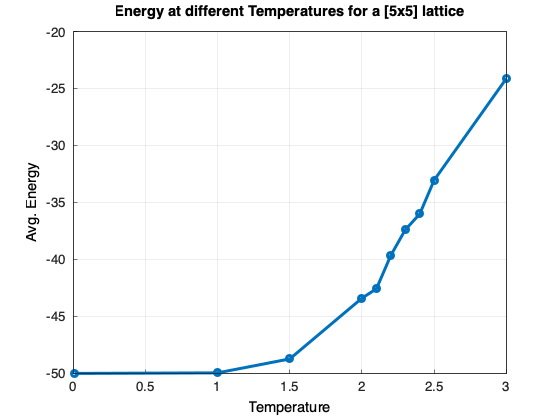
\includegraphics[width=\textwidth]{./img/avg_en_5.png}
		\caption{$L=[5\times5]$}
		\label{sfig:sublabel2}
	\end{subfigure}\\
	\begin{subfigure}{0.5\textwidth}
		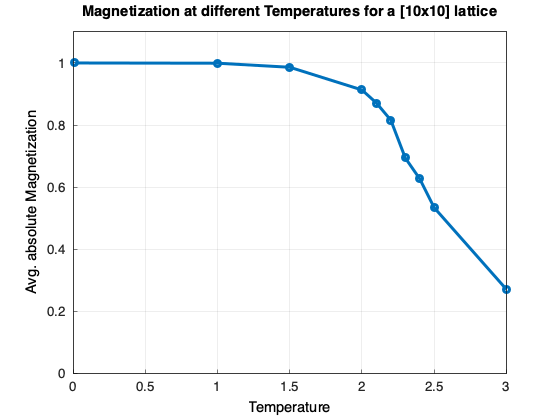
\includegraphics[width=\textwidth]{./img/avg_mag_10.png}
		\caption{$L=[10\times10]$}
		\label{sfig:sublabel3}
	\end{subfigure}%
	~
	\begin{subfigure}{0.5\textwidth}
		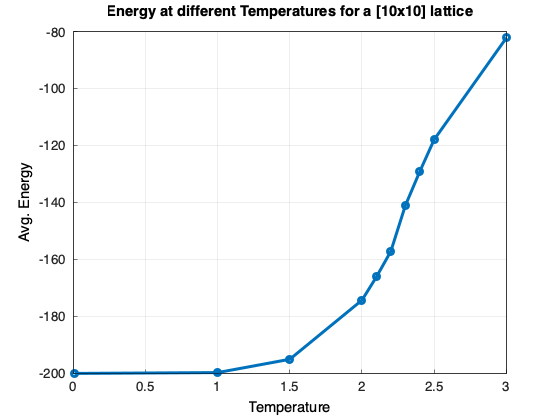
\includegraphics[width=\textwidth]{./img/avg_en_10.png}
		\caption{$L=[10\times10]$}
		\label{sfig:sublabel4}
	\end{subfigure}\\
	\begin{subfigure}{0.5\textwidth}
		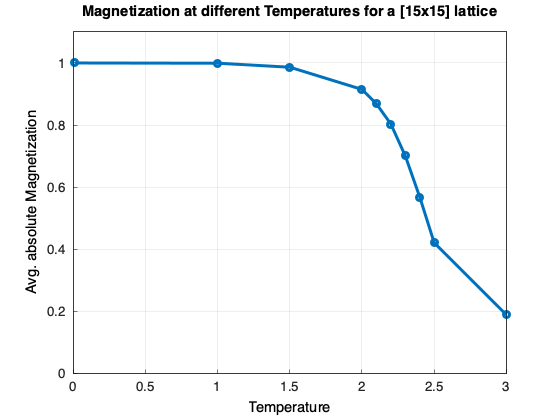
\includegraphics[width=\textwidth]{./img/avg_mag_15.png}
		\caption{$L=[15\times15]$}
		\label{sfig:sublabel5}
	\end{subfigure}%
	~
	\begin{subfigure}{0.5\textwidth}
		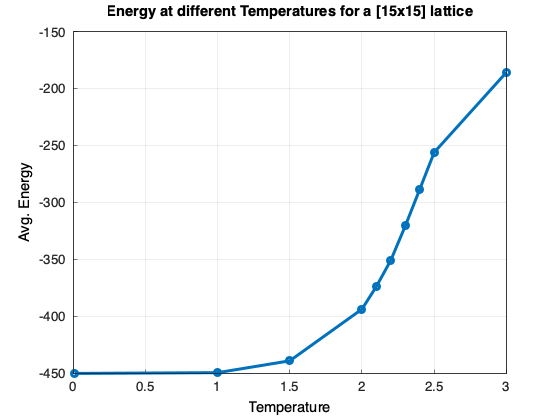
\includegraphics[width=\textwidth]{./img/avg_en_15.png}
		\caption{$L=[15\times15]$}
		\label{sfig:sublabel6}
	\end{subfigure}

	\caption{\textbf{Markov Chains}
		Average absolute magnetization at different temperature is plotted on the left, while on the right the average Energy is plotted versus the temperature.
	}
	\label{fig:avg_em}
\end{figure}
\begin{figure}[t]
	\centering
	\begin{subfigure}{0.5\textwidth}
		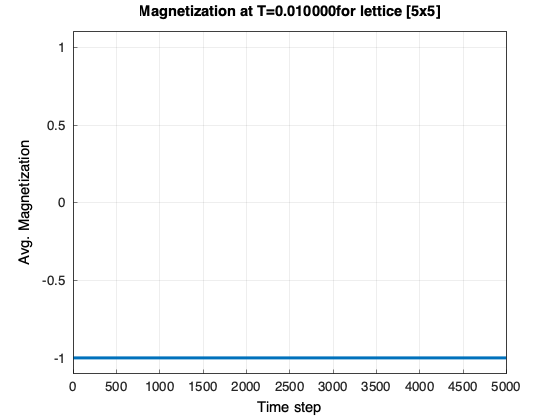
\includegraphics[width=\textwidth]{./img/mag_time_0.010000_5.png}
		\caption{$T=0.01$}
		\label{sfig:p1}
	\end{subfigure}%
	~
	\begin{subfigure}{0.5\textwidth}
		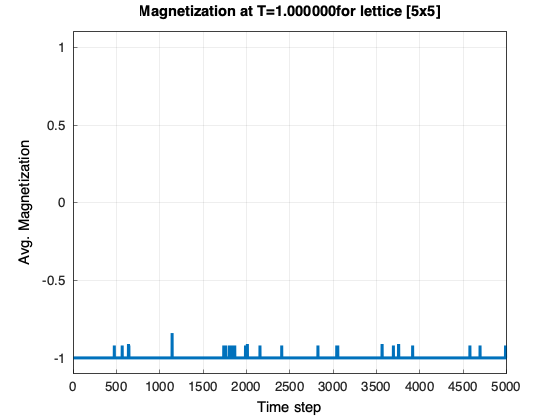
\includegraphics[width=\textwidth]{./img/mag_time_1.000000_5.png}
		\caption{$T=1.0$}
		\label{sfig:p2}
	\end{subfigure}\\
	\begin{subfigure}{0.5\textwidth}
		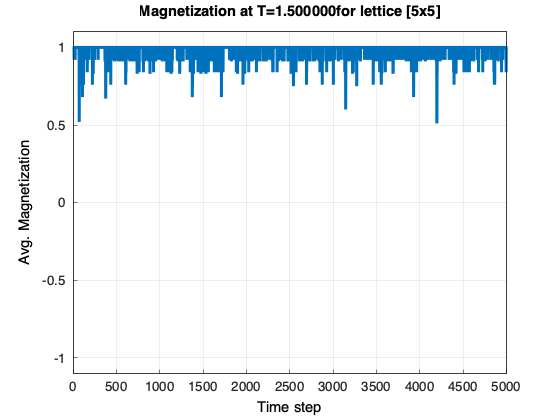
\includegraphics[width=\textwidth]{./img/mag_time_1.500000_5.png}
		\caption{$T=1.5$}
		\label{sfig:p3}
	\end{subfigure}%
	~
	\begin{subfigure}{0.5\textwidth}
		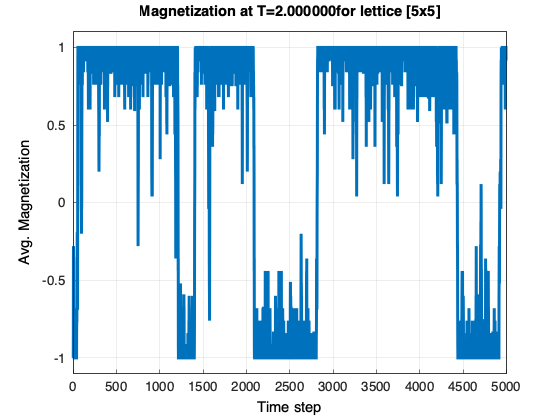
\includegraphics[width=\textwidth]{./img/mag_time_2.000000_5.png}
		\caption{$T=2.0$}
		\label{sfig:p4}
	\end{subfigure}\\
	\begin{subfigure}{0.5\textwidth}
		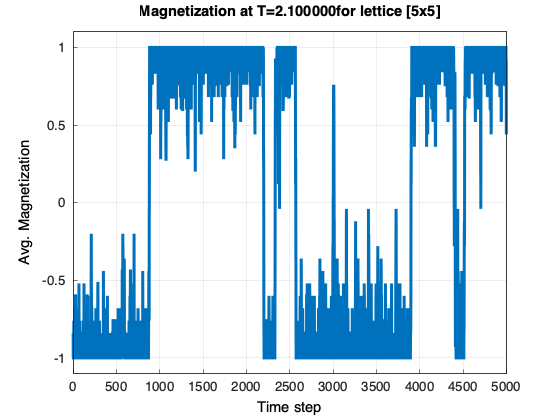
\includegraphics[width=\textwidth]{./img/mag_time_2.100000_5.png}
		\caption{$T=2.1$}
		\label{sfig:p5}
	\end{subfigure}%
	~
	\begin{subfigure}{0.5\textwidth}
		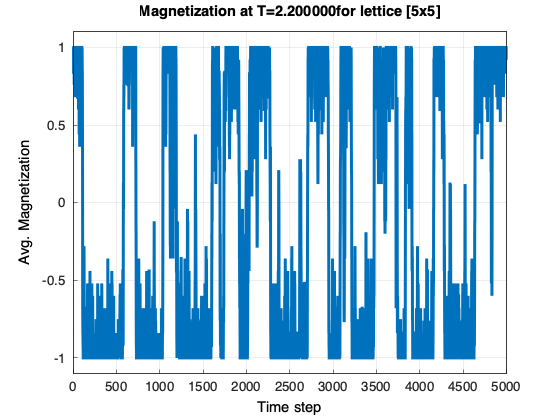
\includegraphics[width=\textwidth]{./img/mag_time_2.200000_5.png}
		\caption{$T=2.2$}
		\label{sfig:p6}
	\end{subfigure}%

	\caption{\textbf{Dependence of $M$ on the simulation time at temperature $T < T_C$}
	}
	\label{fig:mag_time}
\end{figure}
The plots in Figure~\ref{fig:mag_time} show the Ising model simulated on a $5 \times 5$ lattice at different temperatures. (Note that every system was initialized randomly, thus sign between subplots can change as seen in Subfigure \ref{sfig:p3} compared to \ref{sfig:p1} or \ref{sfig:p2}).
We can observe the following behaviour in regards to magnetization sign flips:
\begin{itemize}
	\item Subfigure~\ref{sfig:p1} At temperature close to zero the magnetization is at $-1$ with no sign-flips. All the signs are aligned and there's not enough thermal energy overcome the exchange interaction.
	\item Subfigure~\ref{sfig:p2} The system maintains mostly a magnetization of $-1$, but we can observe occasional small deviations. No sign flips can be seen.
	\item Subfigure~\ref{sfig:p3} More significant deviations appear, yet no sign flips appear. 
	\item Subfigure~\ref{sfig:p4}. \ref{sfig:p5} and \ref{sfig:p6} here we can clearly see sign flips and when increasing the temperature and approach the $T_c$ the sign flips occur more frequently.
\end{itemize}

